% GNUPLOT: LaTeX picture with Postscript
\begingroup
  \makeatletter
  \providecommand\color[2][]{%
    \GenericError{(gnuplot) \space\space\space\@spaces}{%
      Package color not loaded in conjunction with
      terminal option `colourtext'%
    }{See the gnuplot documentation for explanation.%
    }{Either use 'blacktext' in gnuplot or load the package
      color.sty in LaTeX.}%
    \renewcommand\color[2][]{}%
  }%
  \providecommand\includegraphics[2][]{%
    \GenericError{(gnuplot) \space\space\space\@spaces}{%
      Package graphicx or graphics not loaded%
    }{See the gnuplot documentation for explanation.%
    }{The gnuplot epslatex terminal needs graphicx.sty or graphics.sty.}%
    \renewcommand\includegraphics[2][]{}%
  }%
  \providecommand\rotatebox[2]{#2}%
  \@ifundefined{ifGPcolor}{%
    \newif\ifGPcolor
    \GPcolortrue
  }{}%
  \@ifundefined{ifGPblacktext}{%
    \newif\ifGPblacktext
    \GPblacktexttrue
  }{}%
  % define a \g@addto@macro without @ in the name:
  \let\gplgaddtomacro\g@addto@macro
  % define empty templates for all commands taking text:
  \gdef\gplbacktext{}%
  \gdef\gplfronttext{}%
  \makeatother
  \ifGPblacktext
    % no textcolor at all
    \def\colorrgb#1{}%
    \def\colorgray#1{}%
  \else
    % gray or color?
    \ifGPcolor
      \def\colorrgb#1{\color[rgb]{#1}}%
      \def\colorgray#1{\color[gray]{#1}}%
      \expandafter\def\csname LTw\endcsname{\color{white}}%
      \expandafter\def\csname LTb\endcsname{\color{black}}%
      \expandafter\def\csname LTa\endcsname{\color{black}}%
      \expandafter\def\csname LT0\endcsname{\color[rgb]{1,0,0}}%
      \expandafter\def\csname LT1\endcsname{\color[rgb]{0,1,0}}%
      \expandafter\def\csname LT2\endcsname{\color[rgb]{0,0,1}}%
      \expandafter\def\csname LT3\endcsname{\color[rgb]{1,0,1}}%
      \expandafter\def\csname LT4\endcsname{\color[rgb]{0,1,1}}%
      \expandafter\def\csname LT5\endcsname{\color[rgb]{1,1,0}}%
      \expandafter\def\csname LT6\endcsname{\color[rgb]{0,0,0}}%
      \expandafter\def\csname LT7\endcsname{\color[rgb]{1,0.3,0}}%
      \expandafter\def\csname LT8\endcsname{\color[rgb]{0.5,0.5,0.5}}%
    \else
      % gray
      \def\colorrgb#1{\color{black}}%
      \def\colorgray#1{\color[gray]{#1}}%
      \expandafter\def\csname LTw\endcsname{\color{white}}%
      \expandafter\def\csname LTb\endcsname{\color{black}}%
      \expandafter\def\csname LTa\endcsname{\color{black}}%
      \expandafter\def\csname LT0\endcsname{\color{black}}%
      \expandafter\def\csname LT1\endcsname{\color{black}}%
      \expandafter\def\csname LT2\endcsname{\color{black}}%
      \expandafter\def\csname LT3\endcsname{\color{black}}%
      \expandafter\def\csname LT4\endcsname{\color{black}}%
      \expandafter\def\csname LT5\endcsname{\color{black}}%
      \expandafter\def\csname LT6\endcsname{\color{black}}%
      \expandafter\def\csname LT7\endcsname{\color{black}}%
      \expandafter\def\csname LT8\endcsname{\color{black}}%
    \fi
  \fi
    \setlength{\unitlength}{0.0500bp}%
    \ifx\gptboxheight\undefined%
      \newlength{\gptboxheight}%
      \newlength{\gptboxwidth}%
      \newsavebox{\gptboxtext}%
    \fi%
    \setlength{\fboxrule}{0.5pt}%
    \setlength{\fboxsep}{1pt}%
\begin{picture}(6220.00,3960.00)%
    \gplgaddtomacro\gplbacktext{%
      \csname LTb\endcsname%%
      \put(820,652){\makebox(0,0)[r]{\strut{}$-3.0$}}%
      \csname LTb\endcsname%%
      \put(820,960){\makebox(0,0)[r]{\strut{}$-2.0$}}%
      \csname LTb\endcsname%%
      \put(820,1269){\makebox(0,0)[r]{\strut{}$-1.0$}}%
      \csname LTb\endcsname%%
      \put(820,1577){\makebox(0,0)[r]{\strut{}$0.0$}}%
      \csname LTb\endcsname%%
      \put(820,1885){\makebox(0,0)[r]{\strut{}$1.0$}}%
      \csname LTb\endcsname%%
      \put(820,2194){\makebox(0,0)[r]{\strut{}$2.0$}}%
      \csname LTb\endcsname%%
      \put(820,2502){\makebox(0,0)[r]{\strut{}$3.0$}}%
      \csname LTb\endcsname%%
      \put(820,2810){\makebox(0,0)[r]{\strut{}$4.0$}}%
      \csname LTb\endcsname%%
      \put(820,3118){\makebox(0,0)[r]{\strut{}$5.0$}}%
      \csname LTb\endcsname%%
      \put(820,3427){\makebox(0,0)[r]{\strut{}$6.0$}}%
      \csname LTb\endcsname%%
      \put(820,3735){\makebox(0,0)[r]{\strut{}$7.0$}}%
      \csname LTb\endcsname%%
      \put(932,448){\makebox(0,0){\strut{}$8.5$}}%
      \csname LTb\endcsname%%
      \put(1548,448){\makebox(0,0){\strut{}$9$}}%
      \csname LTb\endcsname%%
      \put(2165,448){\makebox(0,0){\strut{}$9.5$}}%
      \csname LTb\endcsname%%
      \put(2781,448){\makebox(0,0){\strut{}$10$}}%
      \csname LTb\endcsname%%
      \put(3398,448){\makebox(0,0){\strut{}$10.5$}}%
      \csname LTb\endcsname%%
      \put(4014,448){\makebox(0,0){\strut{}$11$}}%
      \csname LTb\endcsname%%
      \put(4630,448){\makebox(0,0){\strut{}$11.5$}}%
      \csname LTb\endcsname%%
      \put(5247,448){\makebox(0,0){\strut{}$12$}}%
      \csname LTb\endcsname%%
      \put(5863,448){\makebox(0,0){\strut{}$12.5$}}%
    }%
    \gplgaddtomacro\gplfronttext{%
      \csname LTb\endcsname%%
      \put(186,2193){\rotatebox{-270}{\makebox(0,0){\strut{}$\ln K$\quad}}}%
      \csname LTb\endcsname%%
      \put(3397,142){\makebox(0,0){\strut{}$T^{-1}~(\si{\per\kelvin})\times\num{1e4}$}}%
      \csname LTb\endcsname%%
      \put(4998,3552){\makebox(0,0)[r]{\strut{}\small$\ln K$ = -21,3267 + 2,2492$\times T^{-1}$ ($r^2$ = 0.9995)}}%
    }%
    \gplbacktext
    \put(0,0){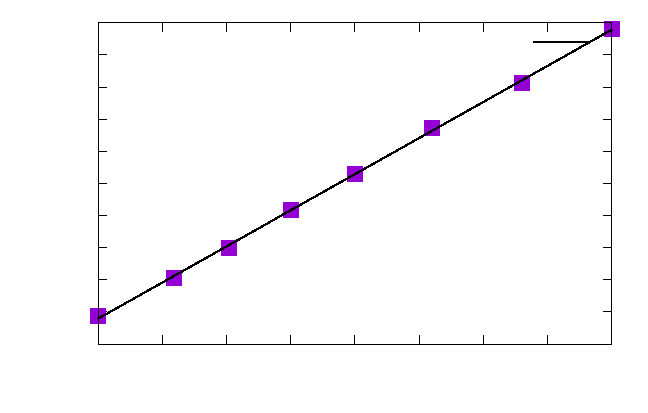
\includegraphics[width={311.00bp},height={198.00bp}]{/home/nicux/Documentos/docencia/repositorio/ejercicios/quimica_general/equilibrio/vant_hoff/figs/vant_hoff}}%
    \gplfronttext
  \end{picture}%
\endgroup
